\documentclass[11pt,a4paper]{article}

\usepackage[margin=2.45cm]{geometry}
\usepackage{amsmath,amssymb,amsthm,mathtools}
\usepackage{booktabs,tabularx,array}
\usepackage{graphicx}
\usepackage{xcolor}
\usepackage{microtype}
\usepackage{hyperref}
\usepackage[numbers,sort&compress]{natbib}
\emergencystretch=1em

\hypersetup{
  colorlinks=true,
  linkcolor=blue!45!black,
  citecolor=blue!45!black,
  urlcolor=blue!45!black,
  pdftitle={Tau Core Physical Source Realization},
  pdfauthor={Jozsef Olcsak}
}

\newtheorem{definition}{Definition}[section]
\newtheorem{theorem}[definition]{Theorem}
\newtheorem{proposition}[definition]{Proposition}
\newtheorem{corollary}[definition]{Corollary}
\newtheorem{lemma}[definition]{Lemma}
\newtheorem{nogo}[definition]{No-go}
\theoremstyle{remark}
\newtheorem{remark}[definition]{Remark}

\newcommand{\Atau}{\mathcal A_\tau}
\newcommand{\Aphys}{\mathfrak A_{\rm phys}}
\newcommand{\Aseed}{\mathfrak A_s}
\newcommand{\Hseed}{\mathcal H_s}
\newcommand{\Hbase}{\mathcal H_B}
\newcommand{\Defsrc}{\operatorname{Def}_{\rm src}}
\newcommand{\Sat}{\operatorname{Sat}_{Bs}}
\newcommand{\Tr}{\operatorname{Tr}}
\newcommand{\id}{\mathbf 1}

\title{\textbf{Tau Core Physical Source Realization:}\\
Complete Seed Presentations, Spectral Selection, and the Nature-Occupation Boundary\\[3pt]
\large An unnumbered technical derivation companion}
\author{Jozsef Olcsak\\Independent researcher}
\date{Version 0.3 --- 28 August 2026}

\begin{document}
\maketitle

\begin{abstract}
The existing Tau Core technical stack begins with a declared physical base
and one universal morphology seed.  We isolate the logically prior question:
under which exact assumptions can a complete relational seed presentation be
realized as a frozen base--seed packet without using terminal observations?
We define an exact source-compatible fibre, a positive Hodge-action operator,
an additive heat-trace complexity, a faithful cyclic spectral state and a
two-sided typed realization certificate.  We then instantiate the input by a
source-frozen P3/CLP3 packet: seven Clifford role generators, two central
record legs, a 256-dimensional cyclic exterior--record representation, a
typed support flag and two ordered cotangent ports.  A min--max argument proves that a
proper finite positive carrier extension with the same frozen compression has
strictly larger heat trace.  Continuity and tensor-product additivity fix the
complexity to a logarithm up to primitive normalization.  Under attainment and
equality-case rigidity the constrained principle selects one
source-equivalence class and exports the input packet required by the
seed--body theorem.  We further construct one nonnegative source-fidelity,
two-sided-Gram and Schur-neutral body-square action.  Once a complete source
language is supplied, this one law jointly realizes premises P4--P7; it cannot
self-certify P1, because an action cannot prove the exhaustivity of the
language in which its own residuals are defined.  We then prove the exact
finite replacement: relative to an independently frozen physical source
algebra with faithful state, P1 is equivalent to full rank of the
seed-generated regular-GNS span.  The present P3/CLP3 control has rank
$256/256$ only relative to its candidate-derived component.  Using instead
the independently declared pre-body PUSC simple envelope gives the conditional
comparison $256/1024=1/4$: if that envelope is ontic and the typed embedding
is physical, P3 is component-complete but not globally exhaustive.  If the
envelope is only an auxiliary metric completion, the physical ambient remains
unidentified.  Hidden spectator, role-rotation, isospectral,
component-zero-jet, nonfaithful-state and off-shell
deformation controls show the exact boundary: the narrow Tau reduct neither
owns the variational priority nor proves that Nature occupies the selected
class.  The result is a conditional physical-source realization calculus, not
a proof of unrestricted parent selection or empirical validation.
\end{abstract}

\begin{center}
\fbox{\begin{minipage}{0.93\linewidth}\small
\textbf{Logical status.}
The theorems below are exact on their declared finite or trace-class domains.
Their physical use additionally assumes that the complete seed grammar, the
Hodge-action unit, the constrained spectral priority and the typed realization
are owned by the physical parent.  Those ownership statements are not derived
from old-bare Tau and are not inferred from readout agreement.  Nature-level
occupation remains open.
\end{minipage}}
\end{center}

\section{Problem and place in the derivation stack}

The generative architecture is required to point forward:
\begin{equation}
 \text{complete seed presentation}
 \longrightarrow \text{physical base--seed packet}
 \longrightarrow M_*
 \longrightarrow \Xi_{OS}
 \longrightarrow Y_a.
 \label{eq:forward}
\end{equation}
The three existing technical companions begin at the second object and derive
body formation, shared observer--source readout and operational terminals.
The purpose of this paper is to type the first arrow.  It neither imports
terminal residuals into the source law nor repeats the downstream theorems.
The foundation architecture and physical-selection boundary are owned by
Foundation Papers I and IV \cite{taupaperI,taupaperIV}.

The output is a data type, not a claim that a specific laboratory endpoint has
already identified its source:
\begin{equation}
 \mathfrak S_*
 =\bigl(B_\tau^{\rm phys},s_U,A_B,J_{\rm seed},N_{\rm phys},
        \mathfrak g_*,\mathcal A_*,\mathcal C_{\rm own}\bigr).
 \label{eq:packet}
\end{equation}
Here $A_B$ is the source-independent base action used by the subsequent body
solve, $J_{\rm seed}$ is its typed seed load, $N_{\rm phys}$ is the retained
physical null policy, $\mathfrak g_*$ is the source-owned grading and
$\mathcal C_{\rm own}$ records which realization premises have actually been
certified.

\begin{figure}[t]
 \centering
 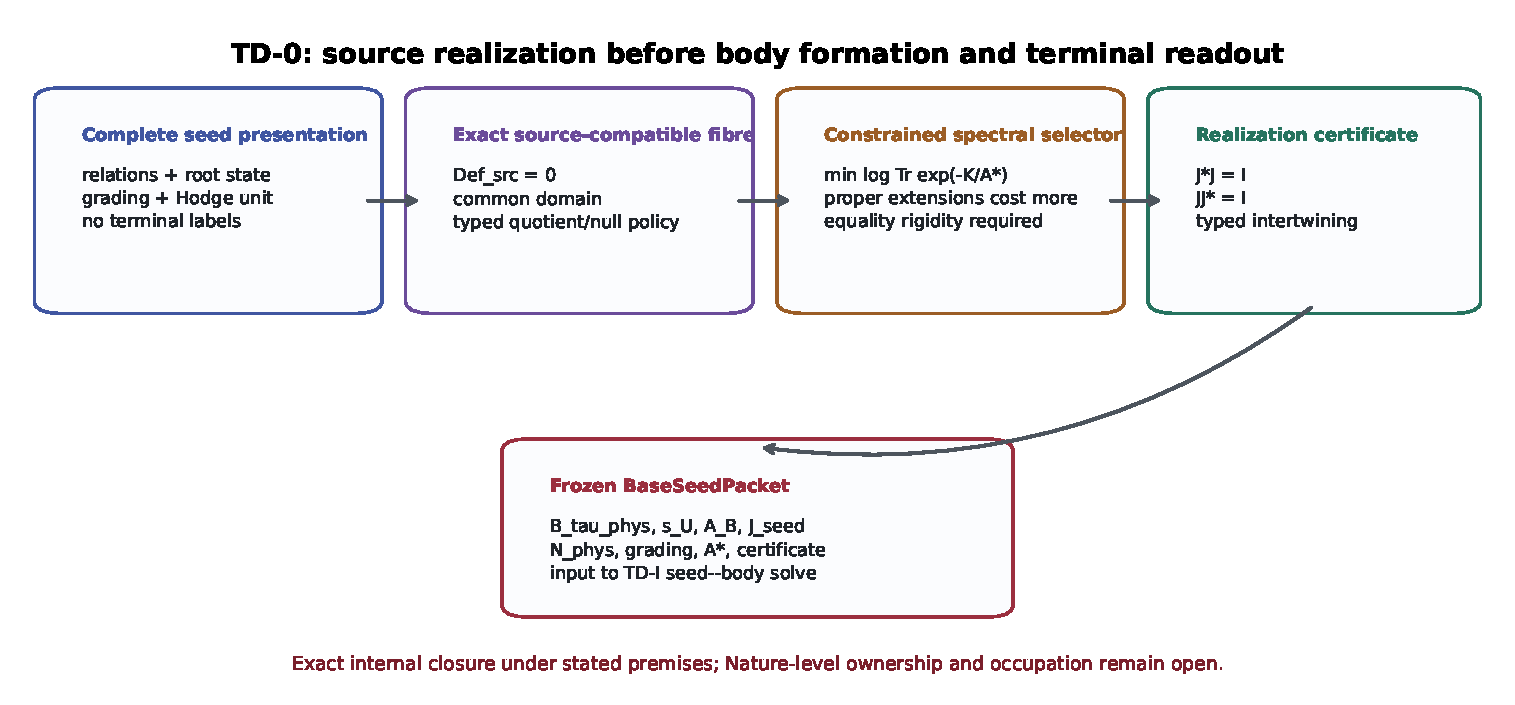
\includegraphics[width=\linewidth]{figures/fig_physical_source_contract.pdf}
 \caption{The TD-0 contract.  Exact source compatibility is imposed before
 spectral minimization; realization precedes body formation; no terminal
 quantity is allowed to select the source packet.}
 \label{fig:contract}
\end{figure}

\subsection{Inherited-results ledger}

\begin{description}
 \item[Foundation Paper I.] Supplies the conditional one-seed,
 joint-law-first input grammar; it does not supply Nature occupation.
 \item[Foundation Paper IV.] Owns the physical parent-selection boundary,
 same-reduct no-go and conditional completion results used here.
 \item[Standard operator algebra.] Supplies the faithful cyclic GNS
 representation theorem used for the occupied source representation.
 \item[Standard spectral theory.] Supplies min--max, interlacing and
 trace-class functional calculus for the extension and state controls.
 \item[Seed--body companion.] Consumes the packet exported here and retains
 ownership of body stationarity and response.
\end{description}
Thus this paper composes established mathematics with declared Tau-side
types; it does not rebrand standard results as Tau theorems.  Nature
occupation has no present theorem owner and remains the stopping boundary.

\section{Typed seed and completion candidates}

\begin{definition}[Complete seed presentation]
A declared complete seed presentation is
\begin{equation}
 \mathfrak S
 =(\mathcal R_s,\Aseed,\pi_s,\Hseed,\Omega_s,
   \mathfrak g_s,\delta_s,\mathcal A_*),
 \label{eq:seedpresentation}
\end{equation}
where $\mathcal R_s$ is the primitive relation set, $\Aseed$ is the generated
unital star algebra, $\pi_s$ is a faithful representation on $\Hseed$,
$\Omega_s$ is a cyclic root, $\mathfrak g_s$ is the typed grading,
$\delta_s$ is a declared Hodge/differential datum and $\mathcal A_*>0$ is one
parent action unit.  Completeness means
\begin{equation}
 \Aseed=C^*\!\left(\pi_s(\mathcal R_s)\right)
 \quad\text{on the declared occupied support.}
 \label{eq:complete}
\end{equation}
It is a premise about source exhaustivity, not a conclusion from the number of
readout channels.
\end{definition}

\begin{definition}[Admissible completion]
An admissible completion of $\mathfrak S$ is
\begin{equation}
 X=(\mathfrak A_X,\pi_X,\mathcal H_X,K_X,\Gamma_X,
     \mathfrak g_X,J_{Xs}),
 \label{eq:candidate}
\end{equation}
where $K_X$ is positive self-adjoint, $\exp(-K_X/\mathcal A_*)$ is trace
class, $J_{Xs}:\Hseed\to\mathcal H_X$ is typed and isometric on the source
support, and the source relations have well-defined residuals
$\rho_\alpha(X;\mathfrak S)$.
\end{definition}

The operator $K_X$ is an atemporal Hodge-action or response-complexity
operator.  It is not a Hamiltonian generating parent time.  Its units are
action, so $K_X/\mathcal A_*$ is dimensionless.  The trace-class and spectral
facts used below are standard \cite{simon2005,reed1978}.

\section{A concrete source-frozen P3/CLP3 presentation}

The generic type above is nonempty in a stronger sense than an abstract
existence claim.  The current P3 construction supplies the following finite
presentation on the declared connected P3 support.  Let
\begin{equation}
 E_{P3}=\operatorname{span}_{\mathbb C}
 \{e_B,e_O,e_R,e_U,e_Q,e_M,e_G\},
 \qquad K_*=I_7,
 \label{eq:p3carrier}
\end{equation}
and let the free unital star algebra be generated by seven self-adjoint
$g_a$ and two central record idempotents $p_0,p_1$.  Quotient by
\begin{align}
 \{g_a,g_b\}&=2\delta_{ab}\id,
 &p_rp_s&=\delta_{rs}p_r,
 &p_0+p_1&=\id,
 &[p_r,g_a]&=0.
 \label{eq:p3relations}
\end{align}
The resulting source algebra is
\begin{equation}
 \Aseed^{P3}
 =\operatorname{Cl}(E_{P3},K_*)\otimes(\mathbb C\oplus\mathbb C)
 \simeq M_8(\mathbb C)^{\oplus4},
 \qquad \dim_{\mathbb C}\Aseed^{P3}=256.
 \label{eq:p3algebra}
\end{equation}
This is a complete presentation on its declared support: the role generators
and record idempotents generate the entire quotient, rather than a proper
terminal-visible subalgebra.

One faithful cyclic realization is
\begin{align}
 \Hseed^{P3}&=\Lambda^\bullet\mathbb C^7\otimes\mathbb C^2_{\rm rec},
 &\dim\Hseed^{P3}&=256,\label{eq:p3hilbert}\\
 \pi_s(g_a)&=(\varepsilon_a+\iota_a)\otimes I_2,
 &\pi_s(p_r)&=I_{128}\otimes|r\rangle\!\langle r|,\label{eq:p3rep}\\
 \Omega_s&=|\varnothing\rangle\otimes
 { |0\rangle+|1\rangle\over\sqrt2}.
 \label{eq:p3root}
\end{align}
The 128 ordered Clifford words send the empty exterior word to a basis of
$\Lambda^\bullet\mathbb C^7$; the two record projectors double this orbit to
rank 256.  Hence $\Omega_s$ is cyclic and the representation is faithful.
The grade involution $g_a\mapsto-g_a$ and record exchange
$p_0\leftrightarrow p_1$ uniquely balance the four simple blocks, giving the
faithful normalized trace
\begin{equation}
 \tau_{\rm sym}(A)={1\over4}\sum_{\epsilon=\pm,\,r=0,1}
 \operatorname{tr}_8(A_{\epsilon r}).
 \label{eq:p3trace}
\end{equation}

For a fully explicit atemporal source weight we freeze
\begin{equation}
 K_s=N_{\rm ext}\otimes I_2,
 \qquad
 Z_s=\Tr e^{-K_s}=2(1+e^{-1})^7.
 \label{eq:p3hodge}
\end{equation}
This is a dimensionless source normalization with $\mathcal A_*=1$.  It is
not a temperature and does not identify the physical action line with
$\hbar$; that identification remains conditional on the separately owned
faithful phase character.

The terminal semantics are not read from the spectrum.  On the relative
six-dimensional source carrier with ordered basis $(B,O,R,Q,M,G)$ we freeze
three commuting support projectors with supports
\begin{equation}
 \{B,M,G\},\qquad\{O,Q\},\qquad\{R,M,G\}.
 \label{eq:p3flag}
\end{equation}
Their simultaneous multiplicities are $1,2,1,2$, yielding the intrinsic
blocks $L_B\oplus W_{OQ}\oplus L_R\oplus W_{MG}$.  The two source-owned
ordered contrast ports
\begin{equation}
 c_{OQ}={e_O-e_Q\over\sqrt2},
 \qquad
 c_{MG}={e_M-e_G\over\sqrt2}
 \label{eq:p3ports}
\end{equation}
split the two planes; the independent unit line $L_U$ raises the rank from six
to seven.  Thus the role labels are supplied by a typed source packet, not by
post-hoc terminal naming.

The component-local extension is represented only up to its physically
identifiable class:
\begin{equation}
 \widehat\Gamma_{\rm CLP3}=\sum_{C\in\pi_0(s_U)}\widehat\Gamma_C,
 \qquad
 \widehat\Gamma_{C_{P3}}=\mathcal L_{P3}^{\min}.
 \label{eq:clp3}
\end{equation}
Primitive-support exhaustivity, component preservation, once-counting,
common-unit realization and an attainable P3 zero are the five simultaneous
JLC clauses.  Under them the law occupies the rank-seven packet and gives
Cartesian/tensor composition only between parent-relation-free components.
The higher-order deformation
$\widehat\Gamma_{\rm CLP3}+\lambda\widehat\Gamma_{\rm CLP3}^2$ has the same
minimum and normal Hessian, so the claim concerns a completion class, not one
observable off-shell polynomial.

\begin{theorem}[Finite P3/CLP3 instantiation certificate]
The source-frozen packet defined by
\eqref{eq:p3carrier}--\eqref{eq:clp3} satisfies the algebraic, cyclicity,
trace, Hodge, support, port and component-local premises of a
\emph{CompleteSeedPresentation} on the declared finite P3 support.  It
therefore supplies a nonempty conditional input to the TD--0 theorem.
\end{theorem}

\begin{proof}
The reproducibility audit constructs the seven Clifford matrices, verifies all
49 anticommutators and rank 128 of their ordered word algebra, constructs the
rank-256 exterior--record root orbit, checks the closed heat trace, recovers
the $1+2+1+2$ simultaneous support decomposition and two orthonormal ports,
and checks the component direct sum and Q/G one-copy fanout.  A hidden
diagonal has full Q and G marginals but only half the joint rank, so it fails
the JLC/LC factorization and is not a second realization of the same complete
packet.  All checks use only the frozen source file.
\end{proof}

The immutable declaration is distributed in the package's derived-data
directory; its SHA--256 fingerprint is recomputed during reproduction.  The
associated audit currently passes 30 of 30 checks.

\subsection{P1--P7 status for this instantiation}

\begin{center}
\small
\begin{tabularx}{\linewidth}{@{}lXX@{}}
\toprule
Premise & Closed on the frozen mathematical witness & Physical/Nature status\\
\midrule
P1 & complete P3 presentation exists & physical ownership not proved\\
P2 & exact finite zero fibre is nonempty & ambient exhaustivity open\\
P3 & $K_s\ge0$ and $e^{-K_s}$ is faithful trace class & closed on finite support\\
P4 & spectral priority is declared endpoint blind & Nature ownership not proved\\
P5 & displayed class has an attained representative & unrestricted equality rigidity open\\
P6 & identity gives a two-sided typed finite witness & physical base ownership not proved\\
P7 & a unit quadratic TD--I interface witness exists & physical body law not selected\\
\bottomrule
\end{tabularx}
\end{center}

Consequently the generated downstream object is deliberately marked as a
candidate form of the \texttt{BaseSeedPacket} type.  Promoting it to a physical
packet would silently assume exactly the Nature-selection statement that
remains under investigation.

\section{One source action compressing P4--P7}

The table above still makes P4--P7 look like four unrelated physical choices.
They can instead be realized by one extended-valued, nonnegative parent action
after the complete source grammar in P1 has been supplied.  Let
$\mathcal I_{\Sat}(X)$ be zero for $X\in\Sat$ and $+\infty$ otherwise.  Let
$\widehat\rho_s$ be the embedded faithful source Hodge state, $\rho_X$ the
faithful Hodge state of a candidate completion, and define
\begin{equation}
 \Gamma_{\rm GE}(J)
 =\lVert J^\dagger J-\id_s\rVert_{\rm HS}^2
  +\lVert JJ^\dagger-\id_B\rVert_{\rm HS}^2 .
 \label{eq:gramglobal}
\end{equation}
For a source-independent positive invertible base Hessian $K_B$, neutral base
point $b_0$ and typed seed load $j_B(s)$, set
\begin{align}
 Q_B(b;s)
 &=\frac12\langle b-b_0,K_B(b-b_0)\rangle
   -\langle j_B(s),b-b_0\rangle
   +\frac12\langle j_B(s),K_B^{-1}j_B(s)\rangle \notag\\
 &=\frac12\left\lVert
 K_B^{1/2}\bigl(b-b_0-K_B^{-1}j_B(s)\bigr)
 \right\rVert^2 .
 \label{eq:bodysquare}
\end{align}
The candidate single-source law is
\begin{equation}
 \boxed{
 \mathcal L_{\rm 1src}(X,J,b)
 =\mathcal I_{\Sat}(X)
 +\mathcal A_*D(\widehat\rho_s\Vert\rho_X)
 +\frac{\mathcal A_*}{2}\Gamma_{\rm GE}(J)
 +Q_B(b;s).}
 \label{eq:onesourcelaw}
\end{equation}
Every term has action units: relative entropy and the source-normalized Gram
defect are dimensionless, while $\mathcal A_*$ and $Q_B$ carry action.  The
construction is atemporal.  Its arguments are simultaneous source,
realization and body coordinates, not a stored history or parent trajectory.

\begin{theorem}[Single-action P4--P7 compression]
Assume that (i) P1 supplies a complete source grammar and exact fibre $\Sat$;
(ii) the candidate class contains a source completion $X_s$ with faithful
state $\widehat\rho_s$, and
$D(\widehat\rho_s\Vert\rho_X)=0$ only for the declared Hodge-unitary
source-equivalence class; (iii) a typed two-sided intertwiner exists; (iv)
$K_B$ is source-independent, positive and invertible; and (v) comparisons are
made in one seed-fixed connected Hodge-generated component, or their relative
component characters are independently supplied.  Then the zero set of
\eqref{eq:onesourcelaw} is exactly
\begin{equation}
 X\sim_s X_s,\qquad
 J^\dagger J=\id_s,\qquad JJ^\dagger=\id_B,\qquad
 b=b_0+K_B^{-1}j_B(s).
 \label{eq:onesourcezero}
\end{equation}
Consequently one owned law supplies the positive completion priority P4,
attainment and equality rigidity P5, the two-sided realization P6, and the
regular TD--I body handoff P7 without terminal fitting.
\end{theorem}

\begin{proof}
On $\Sat$, every term in \eqref{eq:onesourcelaw} is nonnegative.  The supplied
source completion, two-sided intertwiner and body solution attain simultaneous
zero.  Hence every global minimizer must make each term vanish separately.
Faithful-state equality gives $X\sim_sX_s$; the two Hilbert--Schmidt squares
give both Gram identities; completing the last square gives the unique body
coordinate in \eqref{eq:onesourcezero}.  Conversely those four conditions
make the action zero.  The minimum of $Q_B$ is zero for every frozen upstream
packet, so the body solve cannot back-select $X$ or $J$.  Its Hessian is the
source-independent $K_B$ and its first variation contains precisely the typed
load $j_B(s)$.  Thus the source/body arrow remains forward.
\end{proof}

The theorem is a compression result, not a Nature theorem.  It says that
P4--P7 need not be four additional primitive laws if the enriched physical
parent owns \eqref{eq:onesourcelaw}.  The action's 23-check finite audit uses
the frozen P3 Hodge spectrum, proper-support extension, two one-sided Gram
controls and two distinct seed loads.  Both body squares have zero reduced
minimum, explicitly checking the no-back-selection claim.

\begin{nogo}[No self-certification of P1]
No action written in a declared residual language can, from that fact alone,
prove that the language is physically exhaustive.  For example,
\begin{equation}
 \Defsrc(x_0,x_1)=x_0^2
 \label{eq:incompletelanguage}
\end{equation}
vanishes at both $(0,0)$ and $(0,1)$ although the second point carries an
undeclared relation coordinate.  More generally, an independently owned
component constant $\Lambda(c)$ leaves the complete local Hodge packet and all
its derivatives unchanged while it can reverse the global minimum.
Therefore \eqref{eq:onesourcelaw} enforces a supplied P1 grammar but cannot
derive P1 from its own zero set.  Physical P1 ownership requires an independent
source-exhaustivity theorem or is part of the primitive enriched source law.
\end{nogo}

The no-go is sharp.  A negative source-fidelity sign selects a proper
source-compatible extension; a one-sided Gram term permits either hidden
target support or collapsed source support; and a nonpositive $K_B$ removes
the unique regular handoff.  These countermodels are generated alongside the
positive witness and are not fitted to a terminal endpoint.

\section{An independent-ambient certificate for P1}

The no-go forbids self-certification but does not make P1 mathematically
untestable.  What is required is a comparison object not defined by the seed
candidate itself.  Let $\Aphys$ be a finite-dimensional unital star algebra
after an independently frozen physical-null quotient, let $\omega$ be a
faithful state on $\Aphys$, and let
$(\pi_\omega,\mathcal H_\omega,\Omega_\omega)$ be its regular GNS representation.
For the candidate relation set $\mathcal R_s$, define the included seed
subalgebra
\begin{equation}
 \Aseed=C^*(\mathcal R_s)\subseteq\Aphys,
 \qquad
 \mathcal K_s=\pi_\omega(\Aseed)\Omega_\omega\subseteq\mathcal H_\omega.
 \label{eq:ambientgns}
\end{equation}

\begin{theorem}[Finite faithful-GNS exhaustivity]
Under the preceding assumptions,
\begin{equation}
 \boxed{
 \mathcal K_s=\mathcal H_\omega
 \quad\Longleftrightarrow\quad
 \Aseed=\Aphys.}
 \label{eq:p1gns}
\end{equation}
Equivalently, for any basis of the seed-generated algebra embedded by the
faithful GNS map,
\begin{equation}
 \operatorname{rank}\operatorname{Vec}_\omega(\Aseed)
 =\dim\Aphys
 \quad\Longleftrightarrow\quad P1
 \text{ holds relative to the supplied ambient algebra.}
 \label{eq:p1rank}
\end{equation}
\end{theorem}

\begin{proof}
Faithfulness makes the map
$\iota_\omega:a\mapsto\pi_\omega(a)\Omega_\omega$ injective, since
$\lVert\iota_\omega(a)\rVert^2=\omega(a^\dagger a)=0$ implies $a=0$.
Finite-dimensional images are closed, so
$\mathcal K_s=\iota_\omega(\Aseed)$ and
$\mathcal H_\omega=\iota_\omega(\Aphys)$.  Equality of the GNS subspaces therefore
holds exactly when the included algebras have equal dimension, hence are
equal.  Writing the embedded seed basis as columns gives
\eqref{eq:p1rank}.  The reverse implication is immediate.
\end{proof}

Three hypotheses are essential.  Omitting one relation lowers the rank inside
the same ambient component.  Adding an occupied direct-sum component leaves
the complete local seed Gram matrix unchanged while increasing
$\dim\Aphys$.  Finally, a state with zero weight on that hidden direction
quotients it away and can make an incomplete seed appear dense; faithfulness
excludes this false positive.  Thus neither a local two-jet nor an arbitrary
nonfaithful readout seminorm is a P1 certificate.

The executable P3/CLP3 control realizes a $256$-column regular-GNS basis on a
declared $256$-dimensional ambient, and its 18 checks verify
\eqref{eq:p1rank}, basis invariance and all three countercontrols.  It is not a
physical P1 certificate because the ambient dimension was read from the same
P3/CLP3 presentation rather than frozen by an independent parent-source
manifest.  The theorem therefore converts the remaining logical gap into a
precise input obligation; it does not hide the gap in a rank calculation.

\section{The pre-body source-envelope separator}

The central parent derivation contains a comparison object that is independent
of the P3 presentation.  Under the declared protected unital source calculus
PUSC-P1, the ten-dimensional pre-body curvature carrier enters one simple
complex Clifford envelope with normalized trace:
\begin{equation}
 \mathfrak A_{\rm PUSC}
 =\operatorname{Cl}_{10}(\mathbb C)
 \simeq M_{32}(\mathbb C),
 \qquad
 \dim_{\mathbb C}\mathfrak A_{\rm PUSC}=32^2=1024.
 \label{eq:puscambient}
\end{equation}
PUSC-P1 is a source-side declaration made before body formation and contains
no P3 terminal data.  It is nevertheless conditional: neither old-bare Tau
nor present evidence proves that Nature owns this envelope.

The P3 component algebra is
\begin{equation}
 \Aseed^{P3}
 \simeq \operatorname{Cl}_{7}(\mathbb C)
       \otimes(\mathbb C\oplus\mathbb C)
 \simeq M_8(\mathbb C)^{\oplus4},
 \qquad
 \dim_{\mathbb C}\Aseed^{P3}=256.
 \label{eq:p3insidepusc}
\end{equation}
There is a unital star embedding of four $M_8(\mathbb C)$ blocks into
$M_{32}(\mathbb C)$ with multiplicity one.  The normalized matrix trace then
restricts to equal central weights $1/4$ on the four P3 blocks.  This proves
mathematical compatibility of the two finite algebras; physical ownership of
the typed embedding remains an additional premise.

\begin{theorem}[P3/PUSC faithful-GNS separator]
Assume that (i) the pre-body PUSC envelope in
\eqref{eq:puscambient} is the ontic physical source algebra after the physical
null quotient, (ii) its normalized trace is the physical faithful state, and
(iii) the preceding typed P3 embedding is source-owned.  Then
\begin{equation}
 \operatorname{rank}\operatorname{Vec}_{\omega}(\Aseed^{P3})=256
 <1024=\dim_{\mathbb C}\mathfrak A_{\rm PUSC}.
 \label{eq:p3puscrank}
\end{equation}
Consequently the P3 presentation is complete on its declared component but
fails global P1 relative to the ontic PUSC envelope.
\end{theorem}

\begin{proof}
The faithful-GNS map is injective, so the dimension of the P3-generated GNS
subspace equals the algebra dimension in \eqref{eq:p3insidepusc}.  The ambient
GNS space has dimension equal to the algebra dimension in
\eqref{eq:puscambient}.  Equation \eqref{eq:p3puscrank} is therefore exact, and
the finite faithful-GNS exhaustivity theorem excludes equality.  Restricting
the comparison to the included P3 algebra recovers component completeness.
\end{proof}

\begin{nogo}[Local P3 data do not select the envelope ontology]
Two interpretations retain the same P3 algebra, trace restriction, local
Gram data and seed action.  In the first, the whole PUSC Clifford envelope is
physical and \eqref{eq:p3puscrank} rejects global P1.  In the second, that
Clifford algebra is only an auxiliary norm/trace completion and the physical
source algebra is a smaller, independently unspecified object.  P3-local data
therefore cannot decide which interpretation is physical.  The first branch
is a conditional global no-go; the second restores ambient
non-identifiability rather than proving global completeness.
\end{nogo}

The later PUSC--PBSE continuation
$\operatorname{Cl}_{16}(\mathbb C)\simeq M_{256}(\mathbb C)$ has algebra
dimension $65536$, but it is not admissible as the upstream P1 comparison:
PBSE is post-body.  Using it to construct the seed premise would reverse the
forward order in \eqref{eq:forward}.  It is retained only as a downstream
consistency control.

\section{Exact compatibility before complexity}

\begin{definition}[Source defect and exact fibre]
For positive source-fixed weights $w_\alpha$ define
\begin{equation}
 \Defsrc(X\mid\mathfrak S)
 =\sum_{\alpha\in I_s}w_\alpha
   \|\rho_\alpha(X;\mathfrak S)\|_\alpha^2,
 \qquad
 \Sat(\mathfrak S)=\{X:\Defsrc(X\mid\mathfrak S)=0\}.
 \label{eq:defect}
\end{equation}
The residual family is complete only if its common zero set is exactly the
declared source-compatible class.  A finite list that misses a seed relation
does not establish completeness.
\end{definition}

This ordering is essential.  One must not trade a source-law violation against
a lower complexity.  The primary relation is therefore a constrained problem,
not an endpoint-weighted scalar sum:
\begin{equation}
 X_*\in\underset{X\in\Sat(\mathfrak S)}{\arg\min}\;C_{\rm HT}(X).
 \label{eq:selector}
\end{equation}

\begin{definition}[Spectral complexity]
For $X\in\Sat(\mathfrak S)$ let
\begin{equation}
 Z_X=\Tr\exp(-K_X/\mathcal A_*),
 \qquad C_{\rm HT}(X)=\log Z_X.
 \label{eq:heatcomplexity}
\end{equation}
No temperature is present.  The exponential is a positive spectral weighting
of atemporal relation modes.
\end{definition}

\section{Why the logarithmic heat trace is the minimal additive scalar}

\begin{proposition}[Additive spectral form]
Suppose a scalar complexity depends only on $Z_X>0$ through a continuous
function $f$, independent composition obeys
\begin{equation}
 K_{X\boxtimes Y}=K_X\otimes\id+\id\otimes K_Y,
 \label{eq:tensork}
\end{equation}
and complexity is additive.  Then
\begin{equation}
 f(Z_XZ_Y)=f(Z_X)+f(Z_Y)
 \quad\Longrightarrow\quad f(Z)=c\log Z.
 \label{eq:cauchy}
\end{equation}
A primitive normalization fixes $c=1$.
\end{proposition}

\begin{proof}
Functional calculus gives
$\exp[-K_{X\boxtimes Y}/\mathcal A_*]
=\exp(-K_X/\mathcal A_*)\otimes\exp(-K_Y/\mathcal A_*)$, hence
$Z_{X\boxtimes Y}=Z_XZ_Y$.  The continuous multiplicative Cauchy equation on
$\mathbb R_{>0}$ has only $f(Z)=c\log Z$.  Fixing one primitive response
normalization fixes $c$.  This proves the functional form, not its physical
ownership.
\end{proof}

The logarithm is therefore not inserted because it resembles entropy.  It is
the continuous additive scalar of a multiplicative trace weight.  Other
selection laws remain possible if additivity or spectral sufficiency is not a
physical premise.

\section{Strict finite extension theorem}

\begin{theorem}[Proper common-compression extensions cost more]
Let $K$ be a positive Hermitian operator on an $n$-dimensional source carrier
$H$.  Let $\widetilde K$ be positive Hermitian on a proper extension
$\widetilde H=H\oplus H_h$ of dimension $n+m$, $m>0$, and assume its
compression to the frozen source carrier is $K$:
\begin{equation}
 P_H\widetilde K\vert_H=K.
 \label{eq:compression}
\end{equation}
Then for every $\mathcal A_*>0$,
\begin{equation}
 \Tr_{\widetilde H}e^{-\widetilde K/\mathcal A_*}
 >\Tr_He^{-K/\mathcal A_*}.
 \label{eq:stricttrace}
\end{equation}
\end{theorem}

\begin{proof}
Write the ordered eigenvalues as
$\widetilde\lambda_1\le\cdots\le\widetilde\lambda_{n+m}$ and
$\lambda_1\le\cdots\le\lambda_n$.  Cauchy interlacing for the compression
gives $\widetilde\lambda_j\le\lambda_j$ for $1\le j\le n$.  Since the
exponential is strictly positive and decreasing,
\begin{align}
 \sum_{j=1}^{n+m}e^{-\widetilde\lambda_j/\mathcal A_*}
 &\ge \sum_{j=1}^{n}e^{-\lambda_j/\mathcal A_*}
   +\sum_{j=n+1}^{n+m}e^{-\widetilde\lambda_j/\mathcal A_*}\\
 &>\sum_{j=1}^{n}e^{-\lambda_j/\mathcal A_*}.
\end{align}
Thus both $Z$ and $\log Z$ strictly increase.  The proof includes coupled
nonsplit extensions; it does not require block diagonality.
\end{proof}

The theorem extends to suitable compact-resolvent form extensions by the
min--max principle when a common closed form domain and trace-class exponential
are available.  It does not compare candidates that change the frozen source
compression, abandon the common domain, or alter the source grammar.

\section{Faithful occupation from positive spectral weight}

\begin{theorem}[Faithful cyclic spectral state]
Let $K_X$ be self-adjoint, bounded below, and let
$e^{-K_X/\mathcal A_*}$ be trace class for $\mathcal A_*>0$.  Then
\begin{equation}
 \rho_X=\frac{e^{-K_X/\mathcal A_*}}{Z_X}
 \label{eq:rho}
\end{equation}
is a positive normalized state with zero kernel on the spectral support.  Its
standard GNS representation has a cyclic root; it is faithful on the quotient
by any genuine representation null.
\end{theorem}

\begin{proof}
The functional calculus gives strictly positive eigenweights
$e^{-\lambda/\mathcal A_*}$ at every finite spectral value.  Trace-class
normalization gives $\Tr\rho_X=1$, and no occupied spectral vector has zero
weight.  The GNS construction supplies a cyclic vector by definition, while
faithfulness follows after quotienting the state null ideal
\cite{gns1947,bratteli1987}.
\end{proof}

This is spectral occupation inside a supplied completion.  It does not prove
that Nature selects the completion itself, and it is not a Gibbs state in
parent time.

\section{Two-sided realization and source completeness}

\begin{definition}[Typed physical realization certificate]
A realization $J_{Bs}:\Hseed\to\Hbase$ is certified on the claimed support if
\begin{align}
 J_{Bs}^\dagger J_{Bs}&=\id_{\Hseed},
 &J_{Bs}J_{Bs}^\dagger&=\id_{\Hbase},
 \label{eq:twosided}\\
 J_{Bs}\pi_s(r)&=\pi_B(r)J_{Bs},
 &J_{Bs}\mathfrak g_s&=\mathfrak g_BJ_{Bs}
 \quad(r\in\mathcal R_s),
 \label{eq:intertwine}\\
 K_BJ_{Bs}&=J_{Bs}K_s.
 \label{eq:hodgeintertwine}
\end{align}
The first identity excludes loss of a seed distinction; the second excludes
hidden occupied base support.  The remaining identities preserve relations,
typing and the action metric.
\end{definition}

\begin{theorem}[Lossless realization]
Under \eqref{eq:twosided}--\eqref{eq:hodgeintertwine}, $J_{Bs}$ is a unitary
typed equivalence on the declared occupied support.  It transports the
spectral state, source metric and relation algebra without an adjustable gain:
\begin{equation}
 \rho_B=J_{Bs}\rho_sJ_{Bs}^\dagger,
 \qquad
 \Aphys=C^*\!\left(J_{Bs}\pi_s(\mathcal R_s)J_{Bs}^\dagger\right).
 \label{eq:transport}
\end{equation}
\end{theorem}

\begin{proof}
The two Gram identities make $J_{Bs}$ a surjective isometry and hence unitary.
The intertwining relations transport functional calculus, so
$e^{-K_B/\mathcal A_*}=J_{Bs}e^{-K_s/\mathcal A_*}J_{Bs}^\dagger$ and the
traces agree.  Algebra generation follows from complete seed generation and
surjectivity.
\end{proof}

Equation \eqref{eq:transport} is the precise version of ``the full common
relational algebra is in the seed.''  It is a theorem given a complete seed
presentation and a two-sided realization.  It is not implied by the phrase
``one universal seed'' alone.

\section{Conditional selector and packet export}

Let $\sim_s$ identify source-equivalent presentations: candidates are
equivalent when a typed unitary fixes the complete seed image, root state,
Hodge-action operator and physical null policy.

\begin{theorem}[Conditional physical-source realization]
Assume:
\begin{enumerate}
 \item[(P1)] the complete seed presentation \eqref{eq:seedpresentation} is
 physically owned;
 \item[(P2)] $\Sat(\mathfrak S)$ is nonempty and its residual family is
 complete;
 \item[(P3)] every candidate has a positive common-domain $K_X$ with
 trace-class exponential;
 \item[(P4)] the physical base minimizes \eqref{eq:heatcomplexity} on the
 exact fibre \eqref{eq:defect};
 \item[(P5)] the minimum is attained and equality implies $\sim_s$;
 \item[(P6)] the minimizing class carries the two-sided typed certificate
 \eqref{eq:twosided}--\eqref{eq:hodgeintertwine};
 \item[(P7)] its source-independent base action and typed seed first variation
 satisfy the regularity assumptions exported to TD-I.
\end{enumerate}
Then one source-equivalence class $[X_*]_s$ is selected and it exports the
frozen `BaseSeedPacket' \eqref{eq:packet}.  No terminal map or endpoint datum is
required.
\end{theorem}

\begin{proof}
P1--P3 define a nonempty exact admissible fibre and a finite complexity on it.
P4--P5 give one minimizing source-equivalence class.  P6 realizes it without
source loss or hidden occupied base support.  P7 supplies the action and first
variation needed by the downstream body stationarity theorem.  Collecting the
typed objects yields \eqref{eq:packet}.  Every dependency is upstream of body
formation and readout.
\end{proof}

The theorem closes mathematical sufficiency.  Premises P1, P4, P5 and P6 are
the physical ownership content; they must not be hidden inside the word
``seed.''

\section{Adversarial controls and non-entailment}

\begin{nogo}[Hidden seed-annihilator block]
Let $X_0$ realize the declared seed on $H$, and let
\begin{equation}
 X_1=X_0\oplus X_h,
 \qquad \pi_1(r)=\pi_0(r)\oplus0
 \quad(r\in\mathcal R_s),
 \label{eq:hidden}
\end{equation}
with a nonzero positive hidden block.  The proper seed restriction of $X_1$ is
identical to that of $X_0$, so the narrow seed reduct cannot distinguish them.
If P4 is owned and the compression is frozen, the strict extension theorem
rejects $X_1$.  Without P4, no such conclusion follows.
\end{nogo}

\begin{nogo}[Spectra do not name terminal roles]
Let a two-dimensional equal-metric role subspace have $K=\kappa\id$.  Every
$U\in U(2)$ satisfies $UKU^\dagger=K$ and leaves $Z$ unchanged, while rotating
the putative terminal projectors.  Hence heat-trace minimization cannot create
time, quantum or gravity labels.  Their grading and port incidence must be
source owned and transported by \eqref{eq:intertwine}.
\end{nogo}

\begin{nogo}[Off-shell representative non-identifiability]
If $\Gamma\ge0$ has physical zero set $\mathcal Z$ and
$D\Gamma\vert_{\mathcal Z}=0$, then for every $\lambda\ge0$,
\begin{equation}
 \widetilde\Gamma_\lambda=\Gamma+\lambda\Gamma^2
 \label{eq:offshell}
\end{equation}
has the same zero set and the same Hessian on $\mathcal Z$.  Body and linear
readout data therefore identify at most a physical completion class, not one
preferred off-shell formula.
\end{nogo}

\begin{nogo}[Isospectral grading ambiguity]
Two candidates may have the same $K$ spectrum and heat trace while carrying
inequivalent seed embeddings or gradings.  P5 must therefore be a rigidity
statement relative to the complete typed source packet, not merely spectral
nondegeneracy.
\end{nogo}

Together these controls establish the strongest current conclusion:
spectral selection can reject an unneeded carrier extension inside a frozen
source class, but cannot supply source completeness, role semantics or its own
physical priority.

\section{Dimensional, null, and limit audit}

\begin{description}
 \item[Dimension.] $[K_X]=[\mathcal A_*]=$ action; otherwise the
 exponential is undefined.
 \item[Sign.] $K_X$ is bounded below and $\mathcal A_*>0$; otherwise no
 positive normalizable spectral weight is available.
 \item[Nulls.] Only a true common representation null may be quotiented;
 terminal-visible hidden directions must be retained.
 \item[Zero source.] $J_{\rm seed}=0$ must return the declared neutral base.
 \item[Tensor limit.] Independent composition must obey
 \eqref{eq:tensork}; otherwise logarithmic uniqueness does not follow.
 \item[Hidden extension.] A proper positive same-compression carrier must
 strictly increase $C_{\rm HT}$.
 \item[Role rotation.] An equal spectrum with changed typing is the control
 for missing grading ownership.
 \item[Body handoff.] The packet is frozen before $M_*$ is solved, which
 forbids readout-to-source circularity.
\end{description}
These are mathematical failure modes, not after-the-fact repairs.

The construction has no Newtonian or GR limit at this layer because geometry
has not yet descended.  Those known limits belong to the terminal module.  A
parent-time limit is equally inapplicable: the ordering here is logical and
generative, not a trajectory in an absolute external time.

\section{Experiment-facing consequences}

The TD-0 paper is upstream of any experiment, but it makes future tests more
decisive.  A paper claiming a source-frozen Tau prediction must now provide:
\begin{enumerate}
 \item an independently frozen ambient physical source algebra, faithful
 state and physical-null quotient if P1 exhaustivity is claimed;
 \item the exact source residual family used to define $\Sat$;
 \item the selected completion class and its equality/rigidity policy;
 \item the source grading, null policy, $\mathcal A_*$ and realization map;
 \item a hash or immutable declaration freezing the resulting
 `BaseSeedPacket' before terminal endpoints are inspected;
 \item the downstream TD-I--TD-III interfaces and the held-out score.
\end{enumerate}
Failure of a downstream prediction rejects that frozen completion on the
tested support.  It does not justify refitting P1--P7 to the same endpoint.

A positive terminal match establishes Nature-level source information only if
competing standard and same-reduct completions do not force the same relation.
Known-limit agreement remains a control.  Conversely, independent evidence
for a hidden occupied seed-annihilator sector, failure of the two-sided Gram
certificate, or an eligible violation of the frozen terminal consequence
would weaken or reject the selected completion.

\section{Claim ledger and current status}

\begin{description}
 \item[Defined and auditable.] The exact source-compatible fibre, provided
 its complete residual family is supplied.
 \item[Proved.] The finite common-compression extension penalty and the
 faithful spectral state.
 \item[Proved conditionally.] The logarithmic additive form, two-sided
 realization, unique source-equivalence class and `BaseSeedPacket' export,
 under the assumptions stated in Sections 4--9.
 \item[Compressed conditionally.] Given P1 and physical ownership of
 \eqref{eq:onesourcelaw}, P4--P7 follow from one nonnegative source law and are
 not independent selector assumptions.
 \item[Disproved from old-bare Tau.] P1--P7 do not follow from the narrow
 reduct; hidden-block and role-rotation controls witness non-entailment.
 \item[Self-certification no-go.] The single source action cannot prove
 that the residual language used in its own definition is complete; P1 remains
 an independent source-language/exhaustivity statement.
 \item[Independent-ambient P1 theorem.] For a supplied finite physical source
 algebra with faithful state, full regular-GNS rank is necessary and sufficient
 for seed-language exhaustivity relative to that ambient.  The P3/CLP3
 $256/256$ control is mathematically complete but physically ineligible
 because its ambient is not independently owned.
 \item[Pre-body separator.] PUSC-P1 supplies an independent
 candidate ambient $\operatorname{Cl}_{10}(\mathbb C)$.  Under the
 envelope-ontic and physical-embedding premises, P3 has faithful-GNS rank
 $256/1024$ and is therefore component-complete but not globally exhaustive.
 The metric-auxiliary interpretation remains indistinguishable from P3-local
 data, and Nature does not presently select either branch.
 \item[Open.] Nature occupation requires independent source evidence or a
 source-frozen discriminator.  A Tau-specific terminal signal belongs
 downstream of TD-III.
\end{description}
Internal closure is therefore separated from physical ownership and empirical
discrimination.

\section{Conclusion}

The readout derivation stack now has an explicit upstream contract.  A
complete seed presentation first defines an exact compatibility fibre; an
independently owned additive spectral principle selects within that fibre; a
faithful cyclic state occupies the selected support; and a two-sided typed
realization exports the frozen base--seed packet used by body formation.  The
finite extension theorem and adversarial controls make the construction
separately testable and prevent terminal success from being used backward as
source selection.

The decisive remaining physical statement is now narrower:
\begin{equation}
 \boxed{\begin{gathered}
 \text{Is the pre-body source envelope ontic or metric-auxiliary,}\\
 \text{and does the occupied seed have faithful full GNS rank}\\
 \text{in the resulting independently owned physical algebra,}\\
 \text{and }\mathcal L_{\rm 1src}\text{ on its physical component?}
 \end{gathered}}
 \label{eq:nature}
\end{equation}
If yes, P4--P7 follow jointly and the TD--I input is fixed without backward
readout selection.  The mathematics establishes this implication and its
countermodels.  It does not answer the Nature question by definition.

\bibliographystyle{unsrtnat}
\bibliography{refs}

\end{document}
